\chapter{Design}
In this chapter we will explain the applications we developed for this work at a high level. We will skip the experiment automation and plot generation parts of the software, since they are either scripts with a couple of loops that run all the configurations we deemed necessary or simply read data from text files and plot them. Instead, we will be focusing on the two ray tracers we built for this work.

\section{Vulkan Ray Tracer}
\subsection{Rasterized}
The rasterized version of the renderer is quite simple in its design, with a single monolithic Application class handling almost everything and a few helper data structures (Vertex, QueueFamilyIndex, SwapchainSupportDetails and UniformBufferObject) for storing and grouping together information. We see an UML class diagram of this application in figure \ref{rasterized-uml}. This instance of the renderer is much bigger than the following ones due to us not relying on almost any external library and having to handle all the low level operations ourselves, thus resulting in a high ammount of initialization functionality. To all this we added one more class that encapsulates all the performance measuring functionality, which we called FramePerformanceCounter.

\begin{figure}[hbt!]
  \centering
  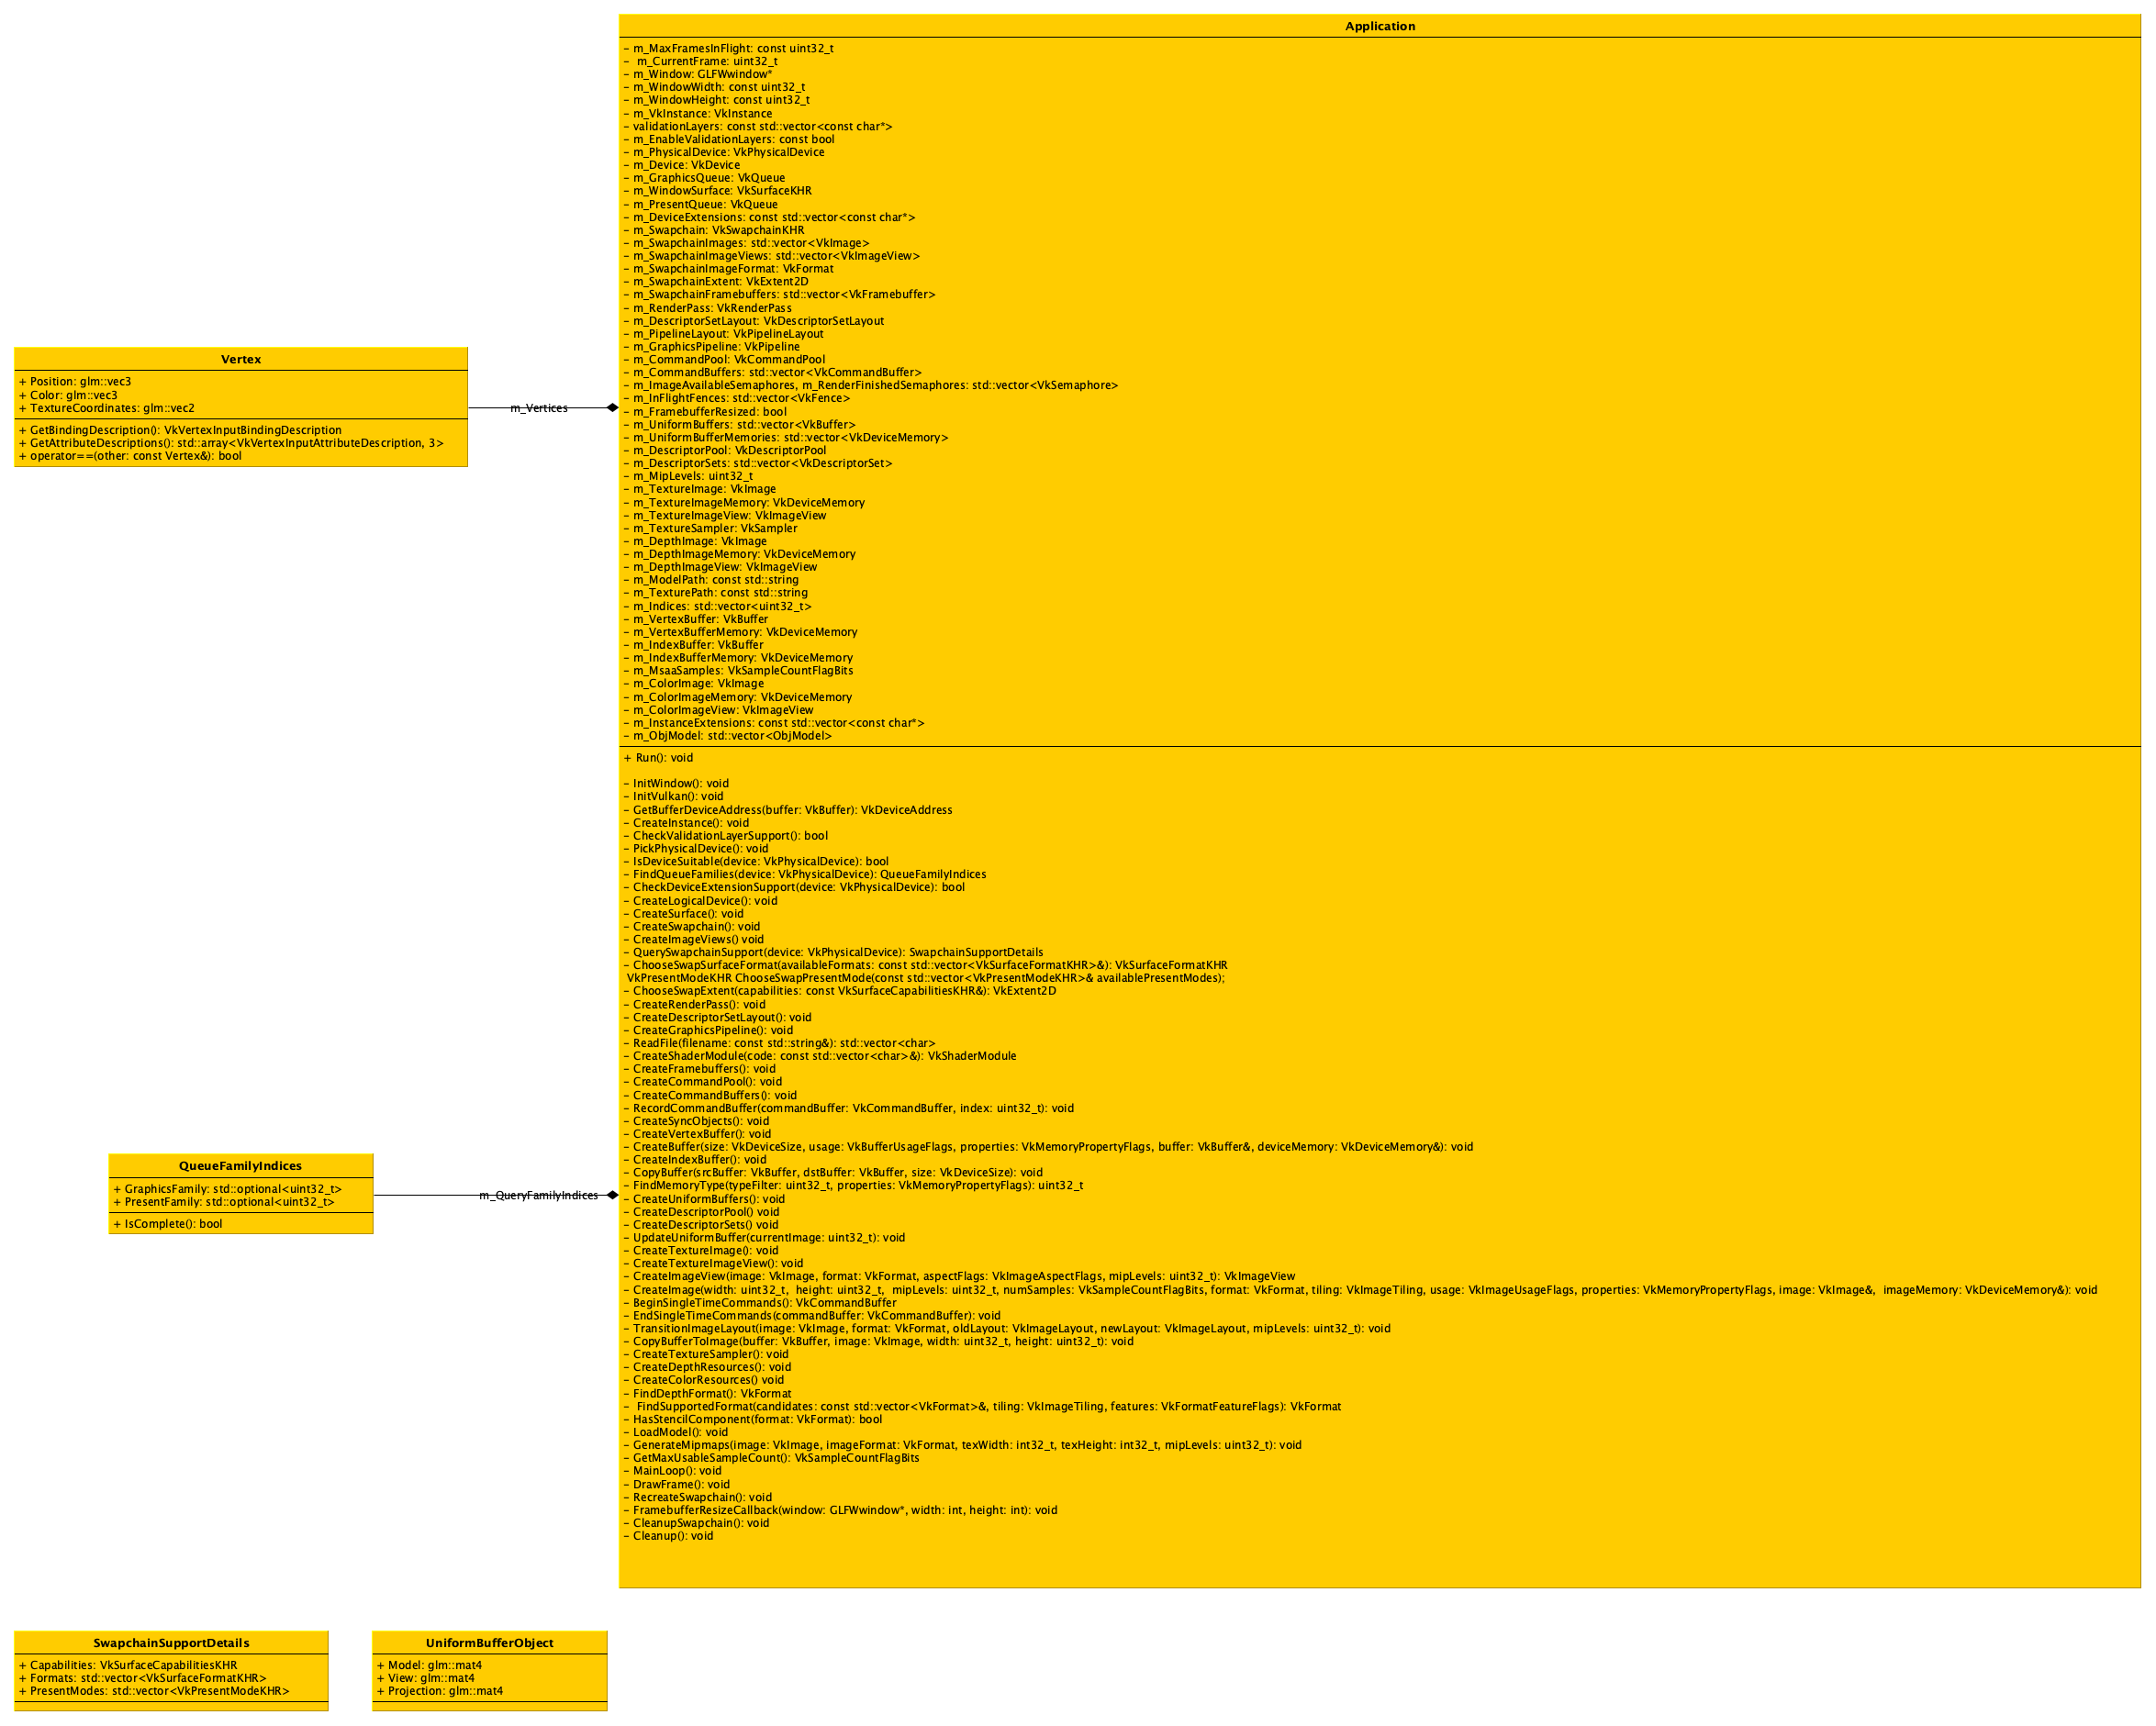
\includegraphics[width=\textwidth]{figuras/rasterized-uml.png}
  \caption{UML class diagram for the rasterized Vulkan renderer.}
  \label{rasterized-uml}
\end{figure}

\subsection{Ray Traced}
For the ray traced version of the Vulkan renderer we refactored and simplified most of the Application class To achieve this, we left an important part of both the initialization and memory cleanup to the Nvvk library. The UML class diagram in figure \ref{vulkan-rt-uml} shows the resulting hierarchy. Finally, we included our own FramePerformanceCounter class for measuring performance.

\begin{figure}[hbt!]
  \centering
  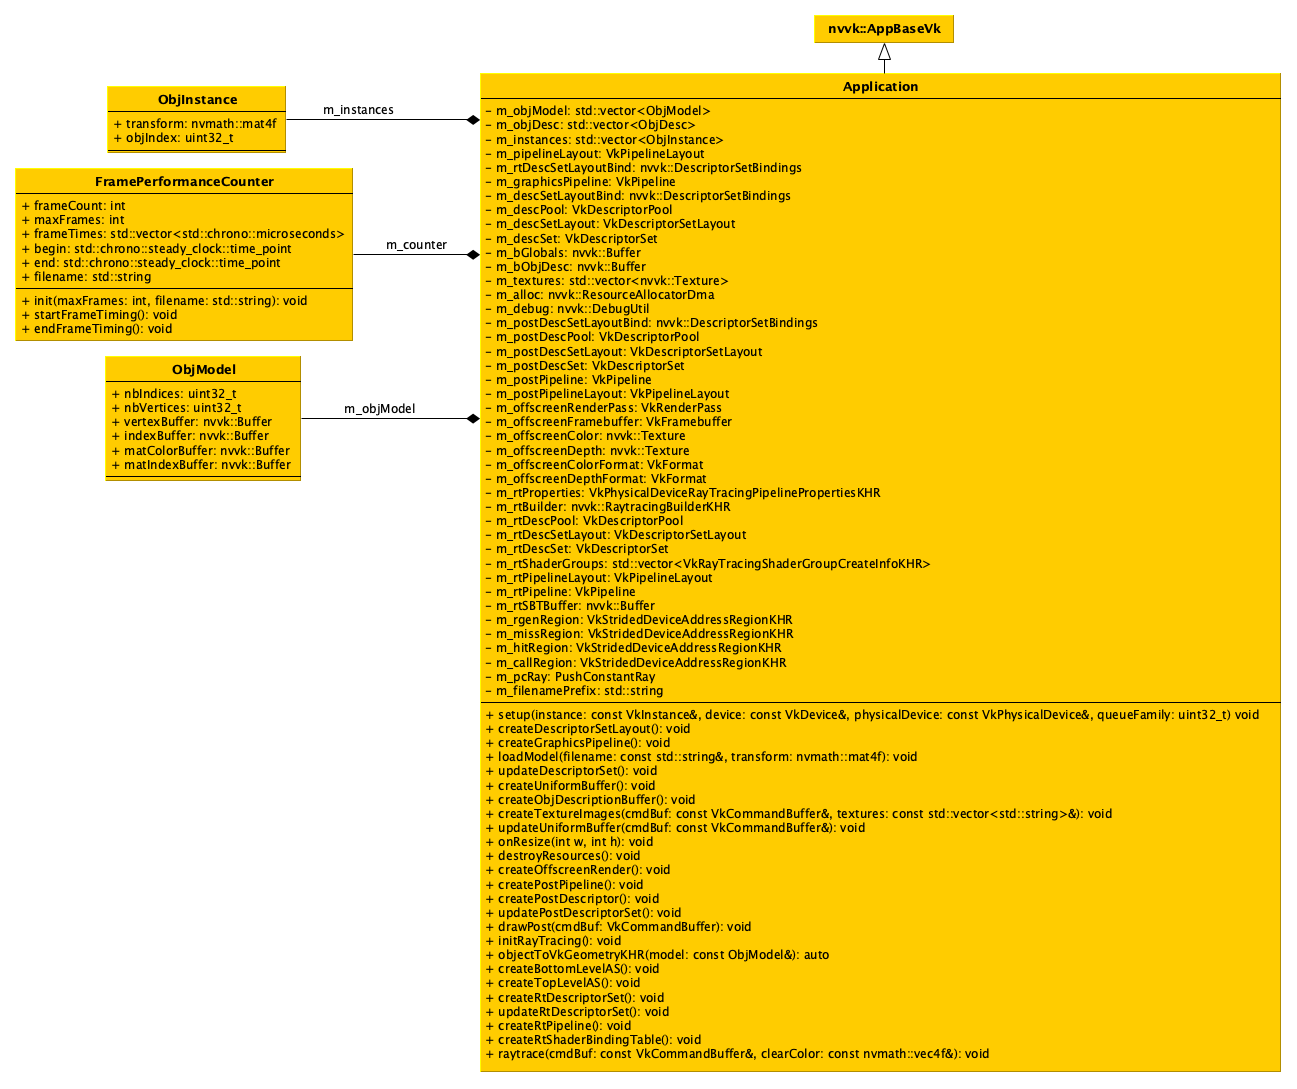
\includegraphics[width=\textwidth]{figuras/vulkan-rt-uml.png}
  \caption{UML class diagram for the raytraced Vulkan renderer.}
  \label{vulkan-rt-uml}
\end{figure}

\section{OptiX Ray Tracer}
For this ray tracer we further encapsulated different functionalities to improve code reusability. This meant increasing the complexity of the class hierarchy. The full diagram can be seen in figure \ref{optix-uml}. 

Here we see a central Renderer class thaat serves much as the Application class from the Vulkan renderer. However, we have encapsulated the window functionality in it's own class hierarchy (GLFWWindow, GLFWCameraWindow). Also, we took the camera manipulation system from the 2019 SIGGRAPH OptiX course \cite{OptixCourse}. This system is highly customizable and perfectly functional, though it adds a fair ammount of complexity to the diagram. This last part includes the classes CameraFrame, CameraFrameManip and it's inheritants. To the class GLFWWindow we also added our FramePerformanceCounter.

\begin{figure}[hbt!]
  \centering
  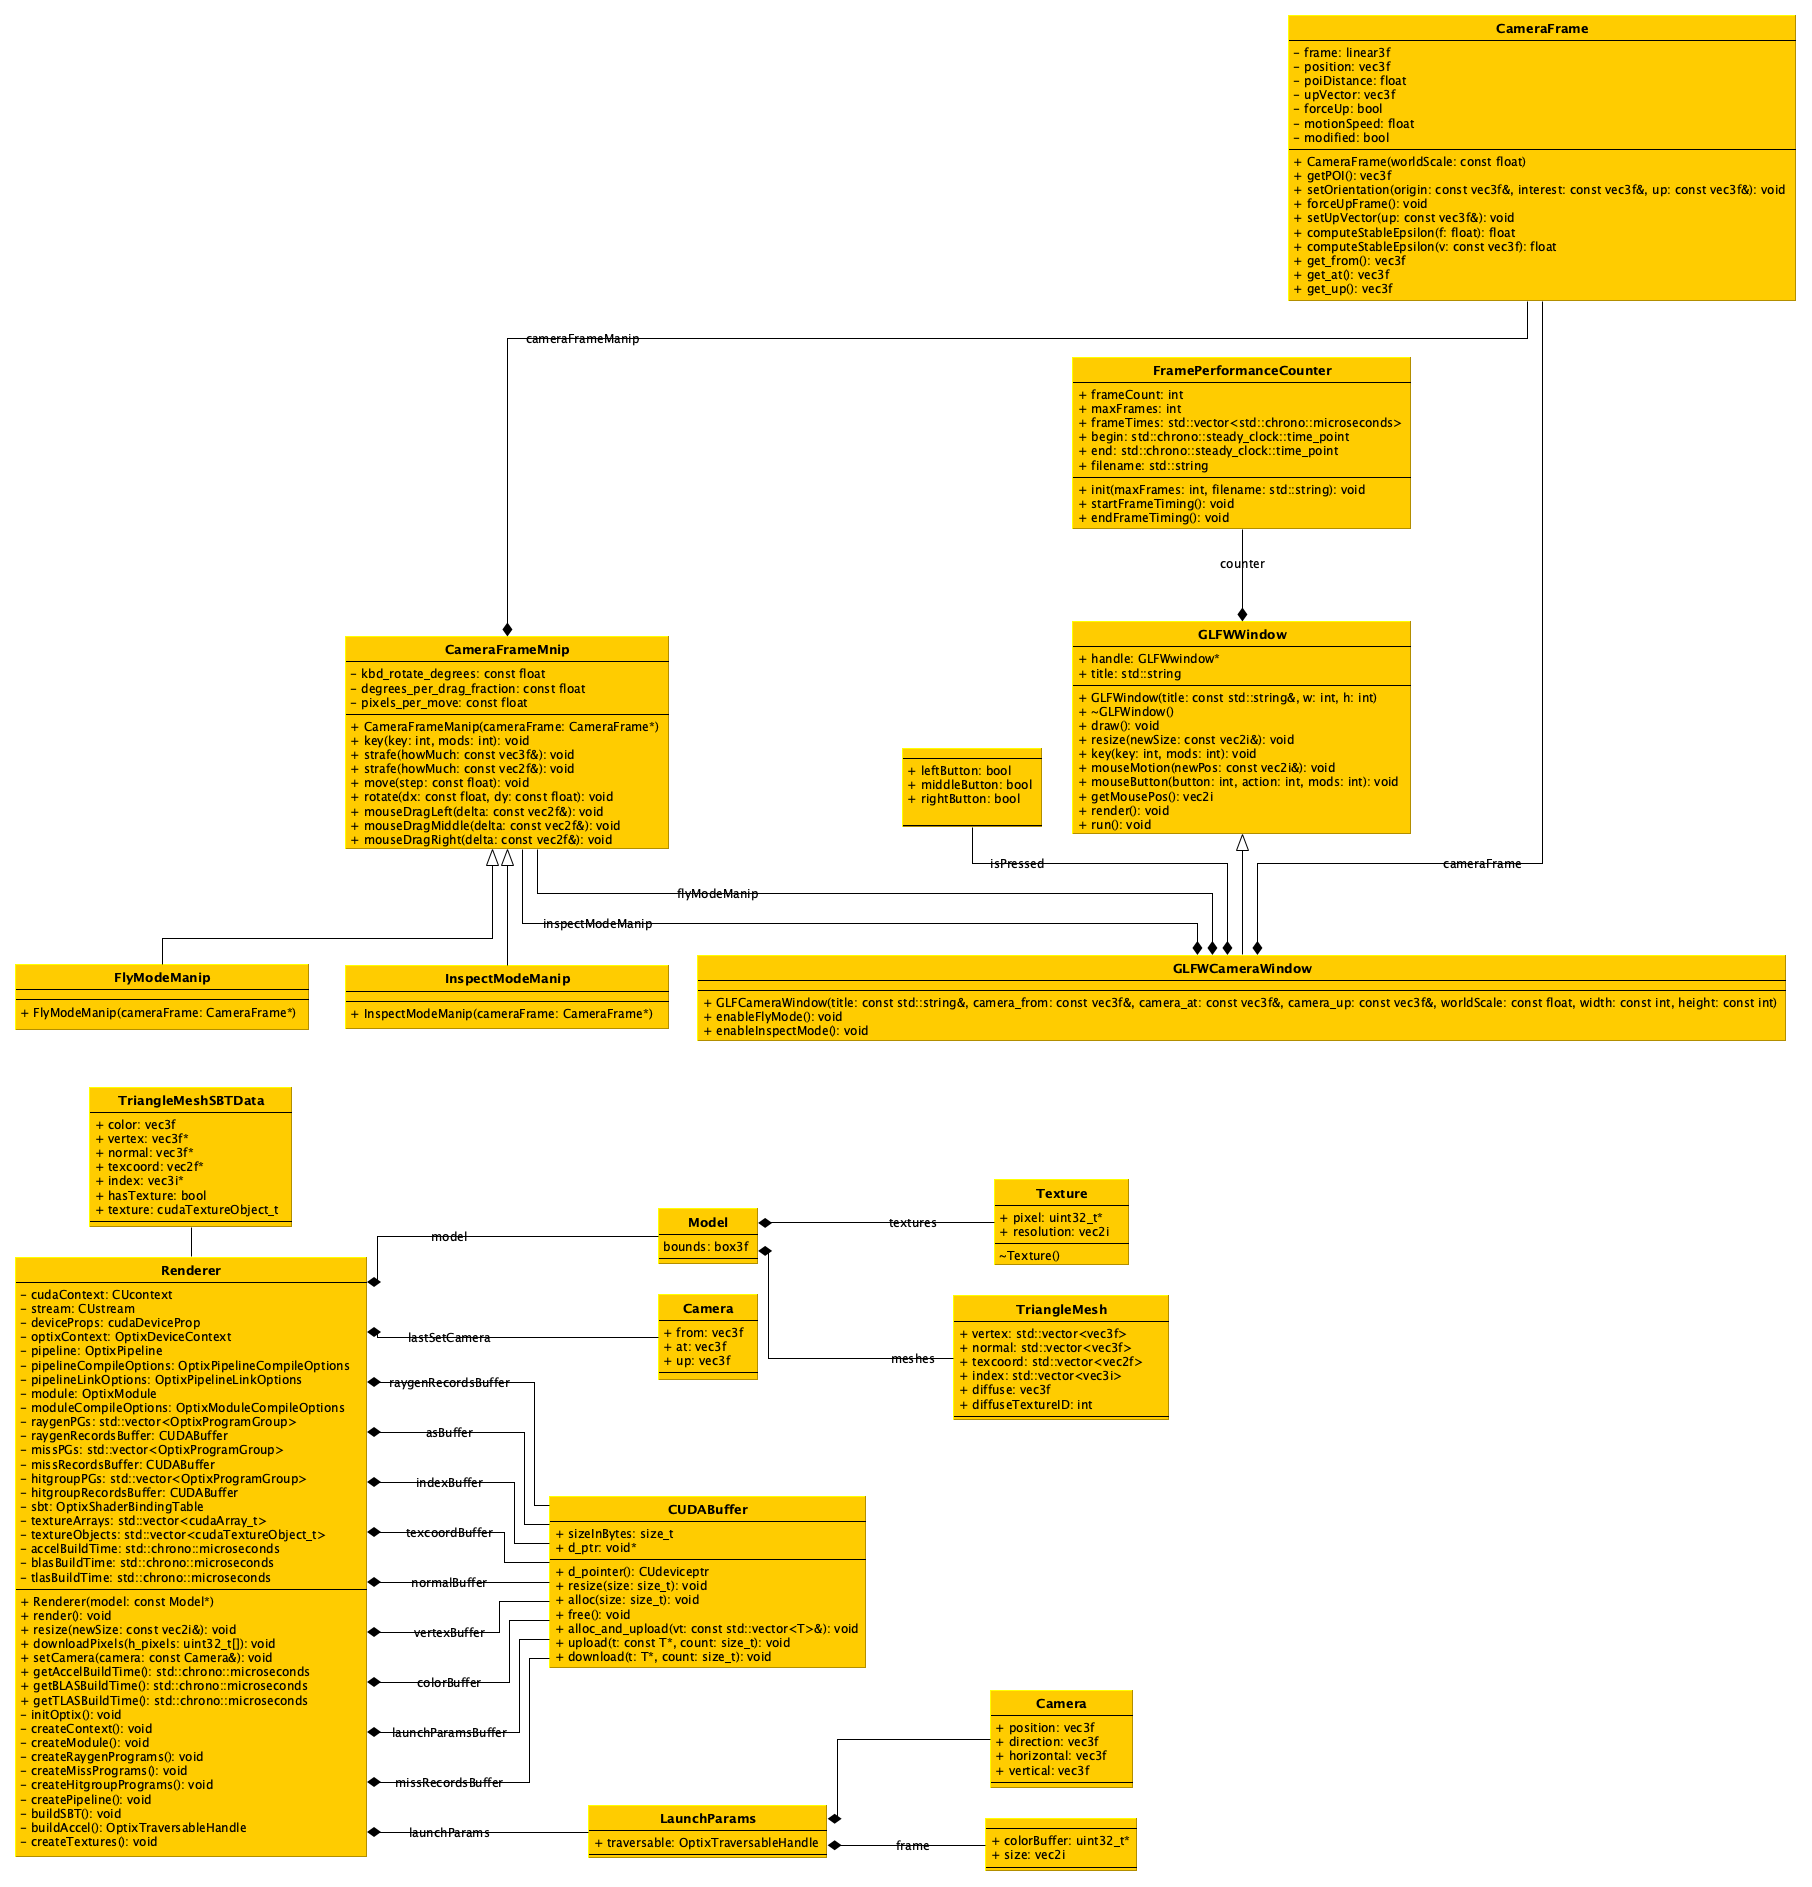
\includegraphics[width=\textwidth]{figuras/optix-uml.png}
  \caption{UML class diagram for the OptiX ray tracer.}
  \label{optix-uml}

\end{figure}
